\documentclass{article}

%\documentclass{report}
\usepackage{braket}
\usepackage{amsmath}
\usepackage{mathtools}
\usepackage{amssymb}
\usepackage{trsym}
\usepackage{pifont}
\usepackage{tcolorbox}
\usepackage[T1]{fontenc}
\usepackage[utf8]{inputenc}
\usepackage[english]{babel}
\usepackage{amsfonts}
\usepackage[super]{nth}
\usepackage{float}
\usepackage{caption}
\usepackage{graphicx}
\usepackage{subcaption}
\usepackage{geometry}
\usepackage{csquotes}
\usepackage{tikz}
\usepackage{circuitikz}
\usepackage{listings}
\usepackage{bbm}
\usepackage{siunitx}
\usepackage{hyperref}
\makeatletter
\renewcommand\paragraph{\@startsection{paragraph}{4}{\z@}%
	{-2.5ex\@plus -1ex \@minus -.25ex}%
	{1.25ex \@plus .25ex}%
	{\normalfont\normalsize\bfseries}}
\makeatother
\setcounter{secnumdepth}{4} % how many sectioning levels to assign numbers to
\setcounter{tocdepth}{4}    % how many sectioning levels to show in ToC
\usetikzlibrary{decorations.pathmorphing}
\geometry{
	a4paper,
	total={150mm,237mm},
	left=30mm,
	top=25mm,
}

\graphicspath{{imgs/}}

\DeclareMathOperator{\var}{Var}

\title{Harmonic Oscillator}
\author{Benedikt Otto}


\begin{document}
	\maketitle
	\newpage
	\tableofcontents
	\newpage
	\begin{abstract}

	\end{abstract}
	\section{Introduction}
	\section{Theoretical Basis}
		To evaluate the behaviour of a quantum particle in a certain potential the path-integral method is used.
		At first the positions of the particle at every time step is initialised to a constant value or a random distribution.
		Then for every time step a new position is drawn from a random distribution, in this case a gaussian distribution.
		If this change lowers the total action, calculated over all the time lattice points, the change is accepted.
		Otherwise, a linearly distributed random value is drawn in the range from 0 to 1 and compared to the exponent of the difference in the Action, divided by a $\hbar$.
		If the random variable is smaller than the exponential function, the value is accepted, otherwise is is rejected and the position at that time step not updated.
		This behaviour leads to the tendency to thermalise, but takes care of the quantum behaviour of the particle.
		\\
		The total action is given by equation \ref{eq:total_action}
		\begin{equation}
			S =
		\end{equation}
	\section{Methods}
	\section{Results}
	\begin{figure}[htbp]
		\centering
		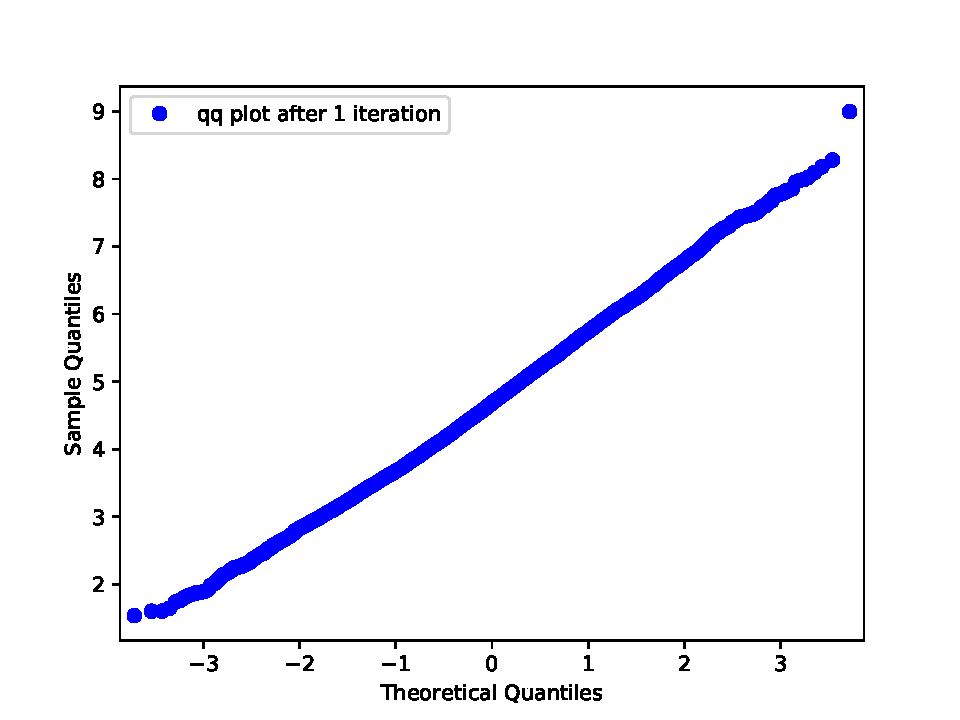
\includegraphics[width=0.4\textwidth]{../imgs/harmonic_oscillator_track/track_10010000_qq_1.pdf}
		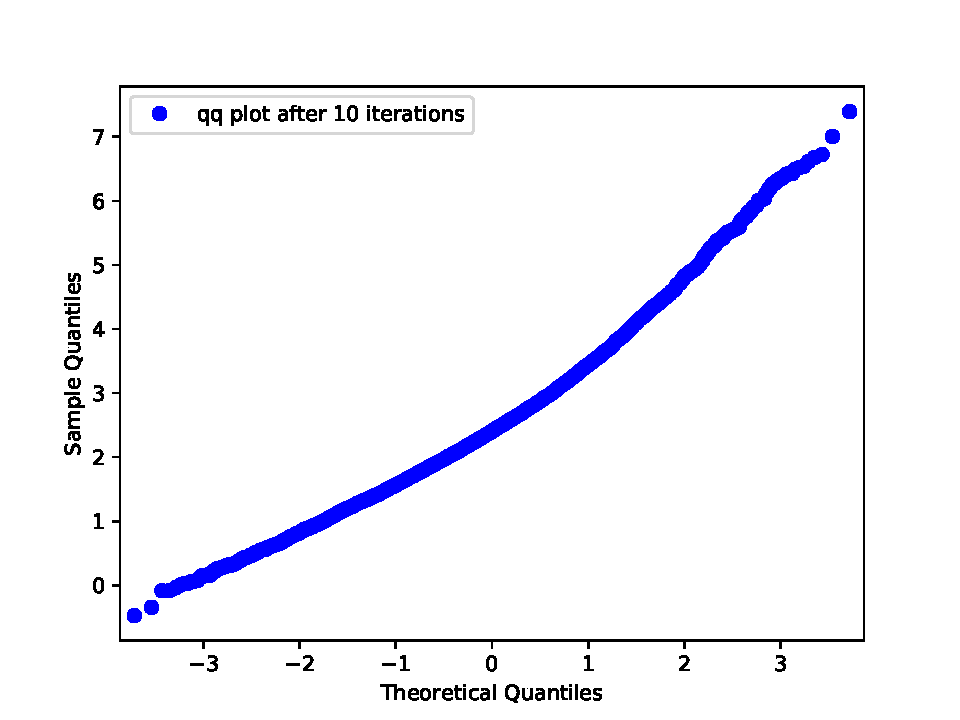
\includegraphics[width=0.4\textwidth]{../imgs/harmonic_oscillator_track/track_10010000_qq_10.pdf}
		\\
		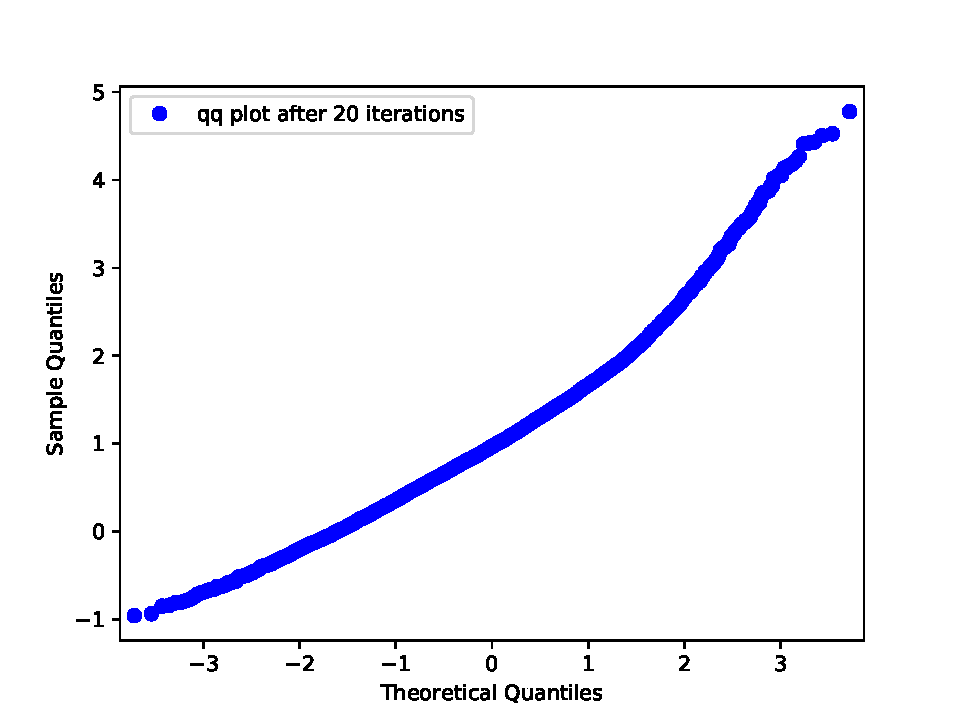
\includegraphics[width=0.4\textwidth]{../imgs/harmonic_oscillator_track/track_10010000_qq_20.pdf}
		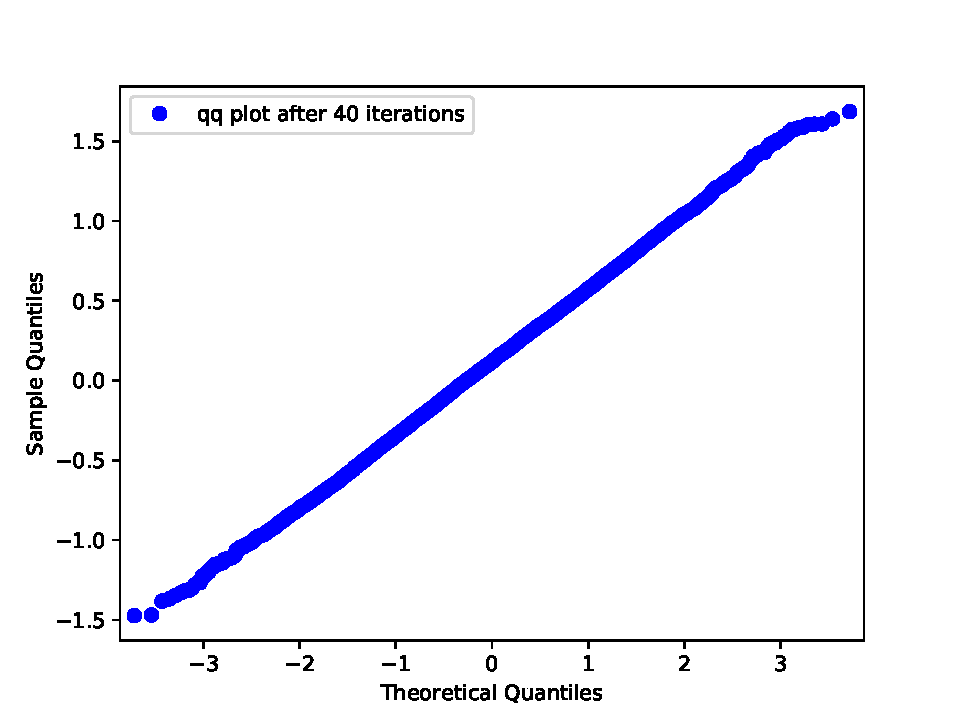
\includegraphics[width=0.4\textwidth]{../imgs/harmonic_oscillator_track/track_10010000_qq_40.pdf}
		\\
		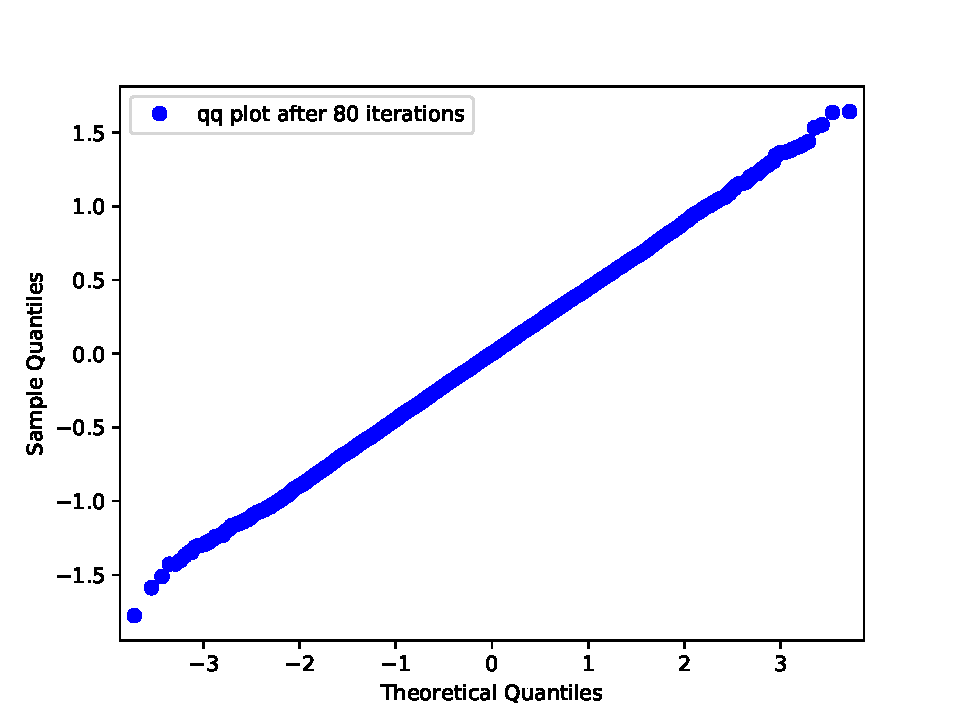
\includegraphics[width=0.4\textwidth]{../imgs/harmonic_oscillator_track/track_10010000_qq_80.pdf}
		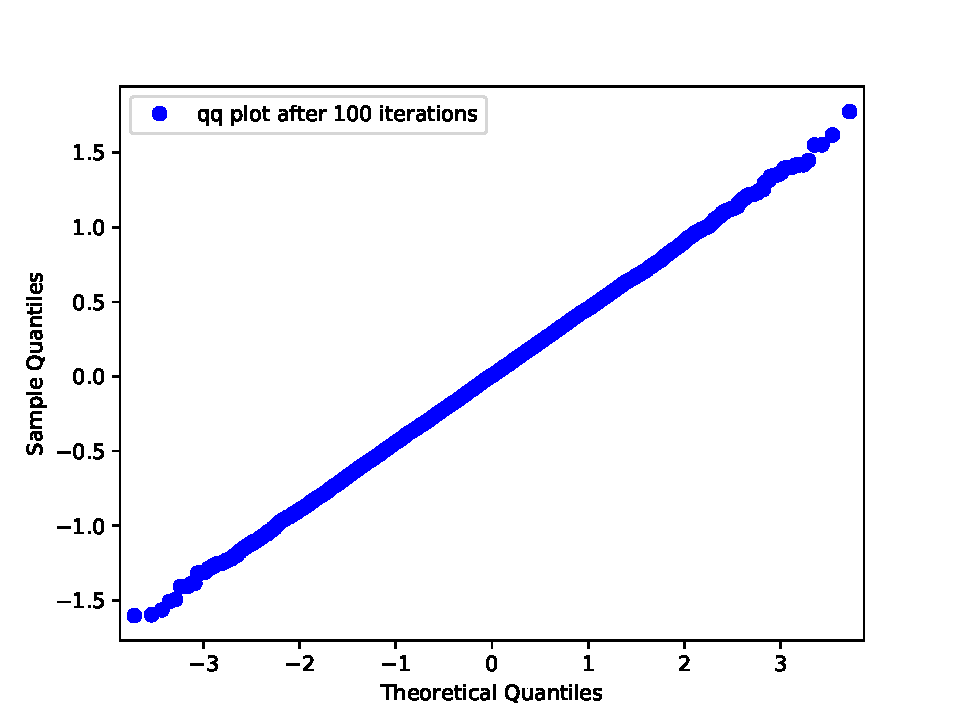
\includegraphics[width=0.4\textwidth]{../imgs/harmonic_oscillator_track/track_10010000_qq_100.pdf}
		\caption{}
	\end{figure}
	\section{Discussion}
	\section{Summary and Outlook}
\end{document}